\apendice{Especificación de diseño}

\section{Introducción}

En este apartado de los anexos, explicaremos la forma que se resolvieron diferentes especificaciones y los casos de uso mencionados en el apartado anterior. Se intentarán analizar el porqué de las tomas de decisiones. Los diseños se dividen en:

\begin{itemize}
	\item Diseño de datos.
	\item Diseño procedimental.
	\item Diseño arquitectónico.
	\item Diseño de interfaz.
\end{itemize}

\section{Diseño de datos}

En este proyecto, los datos que manejaremos serán la creación de usuarios y los contratos que estos creen posteriormente.

Estos datos se almacenarán en una base de datos, aquellos contendrán el id de usuario y este irá relacionado con el resto de elementos de la tabla. Estos elementos les comentaremos a continuación cuando hablemos de la base de datos.



\subsection{Modelo de datos}

En la siguiente figura \ref{fig:modelo} se mostrará el modelo de datos.

\begin{figure}[h!]
    \centering
    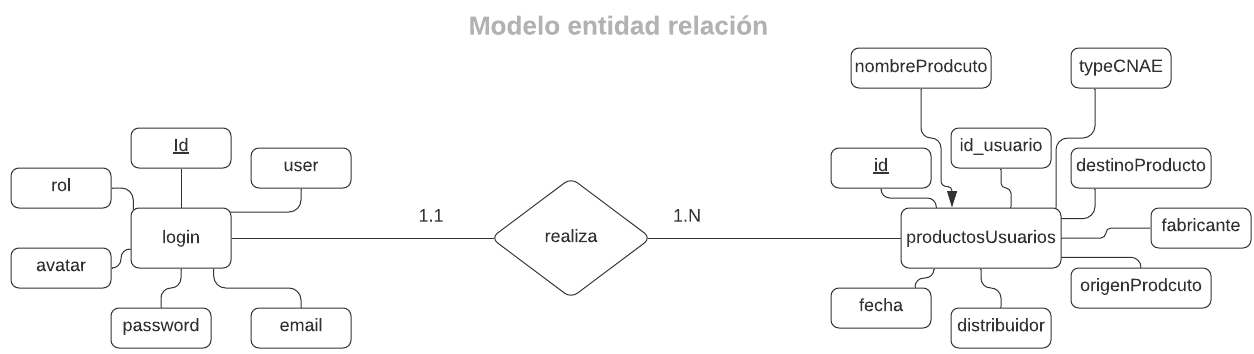
\includegraphics[width=1.00\textwidth]{modeloER}
    \caption{Modelo de datos}
    \label{fig:modelo}
\end{figure}



\subsection{XAMPP}

Utilizaremos una base de datos MySql para el almacenamiento de la información de los datos de nuestra aplicación. La base de datos está compuesta por dos tablas:

\textbf{Usuarios}: en esta tabla almacenaremos la información relacionada con la creación de nuevos usuarios registrados previamente. Esta formado por siete campos, que son los siguientes:
\begin{figure}[H]
    \centering
    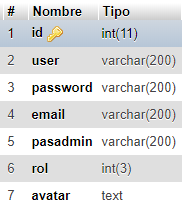
\includegraphics[width=0.60\textwidth]{loginBD}
    \caption{Tabla de usuarios}
\end{figure}
\begin{itemize}
	\item \textit{ID}: es la clave primaria (PK) y almacenará un valor único por cada usuario. Este valor es autoincremental.
	\item \textit{User}: donde se guarda el valor del usuario registrado.
	\item \textit{Password}: guardaremos la contraseña que indicó el usuario, esta a su vez se guardará de forma codificada mediante sha-1.
	\item \textit{Email}: en este campo guardaremos el correo del usuario, el cual será un campo único y, en caso de introducir el mismo, no nos dejará guardarlo de nuevo
	\item \textit{Pasaadmin}: campo diseñado para guardar la contraseña en caso de ser los administradores de la página. Este campo actualmente no está en uso ya que descartamos la opción de poder crear administradores nuevos.  	
	\item \textit{Rol}: tendrá dos posibles valores, dependiendo de si somos los administradores o, por el contrario, somos los usuarios de la página. Los valores sera 1 o 2 respectivamente.
	\item \textit{Avatar}: en el último campo tendremos la foto predeterminada del usuario en caso de que haya seleccionado foto a la hora de registrarse, si no está, será una foto neutra.
\end{itemize}

\textbf{Productos de los usuarios}: en esta nueva tabla se almacenarán todos los productos que el usuario, previamente registrado, ha realizado en la red de Ethereum. Hay un total de diez campos y son los siguientes:
 
\begin{figure}[h]
    \centering
    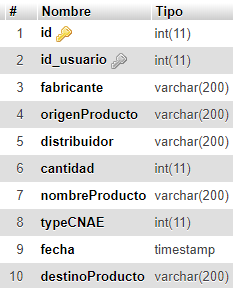
\includegraphics[width=0.80\textwidth]{productoBD}
    \caption{Tabla de productos}
\end{figure}

\begin{itemize}
	\item \textit{Id}: es la clave primaria de la tabla (PK), el valor es auto incremental haciendo que cada producto posea un identificador único.
	\item \textit{Id usuario}: es la clave foránea, la cual se relaciona con la clave primaria de la tabla anterior (usuarios). Gracias a esto tendremos siempre relacionada la tabla usuarios con la de productos, gracias al Id del usuario.
	\item \textit{Fabricante}: indica a quién estamos pidiendo el producto cada vez. Se trata de un campo de caracteres.
	\item \textit{OrigenProducto}: nos referimos de dónde saldrá el paquete en su origen, es un campo de caracteres.
	\item \textit{Distribuidor}: indicaremos quién es el encargado del reparto en cada producto registrado, este campo es de caracteres. 
	\item \textit{Cantidad}: hará referencia al número que queremos adquirir para el pedido de ese producto, este campo es numérico. 
	\item \textit{NombreProducto}: nos referimos al nombre concreto del producto que deseamos adquirir, este campo será de caracteres.
	\item \textit{TypeCNAE}: indicaremos mediante un valor numérico la Clasificación Nacional de Actividades Económicas (CNAE).
	\item \textit{Fecha}: recogeremos la hora en la que se realizó el contrato en nuestra red, este tiempo puede variar unos segundos  la red Ethereum.
	\item \textit{DestinoProdcuto}: es lo mismo que el origenProdcuto, pero esta vez tendremos que indicar el punto final del paquete, es un campo de caracteres.	
\end{itemize}

\section{Diseño procedimental}

En este punto, explicaremos el comportamiento de la aplicación y veremos los procedimientos o funcionalidades que existen en el proyecto. En bases generales esto intenta ser lo más intuitivo y eficaz para que lo pueda usar todo tipo de usuarios.

Contamos con una base de datos ya creada, la cual contará con las dos tablas previamente explicadas, dichas tablas no se podrán modificar.

Tendremos dos tipos de entrada en la página web, podrán ser mediante administrador, o bien, mediante usuario.

La siguiente imagen muestra el diagrama de flujo \ref{fig:diagrama} el inicio de sesión de la página web:

\begin{figure}[H]
    \centering
    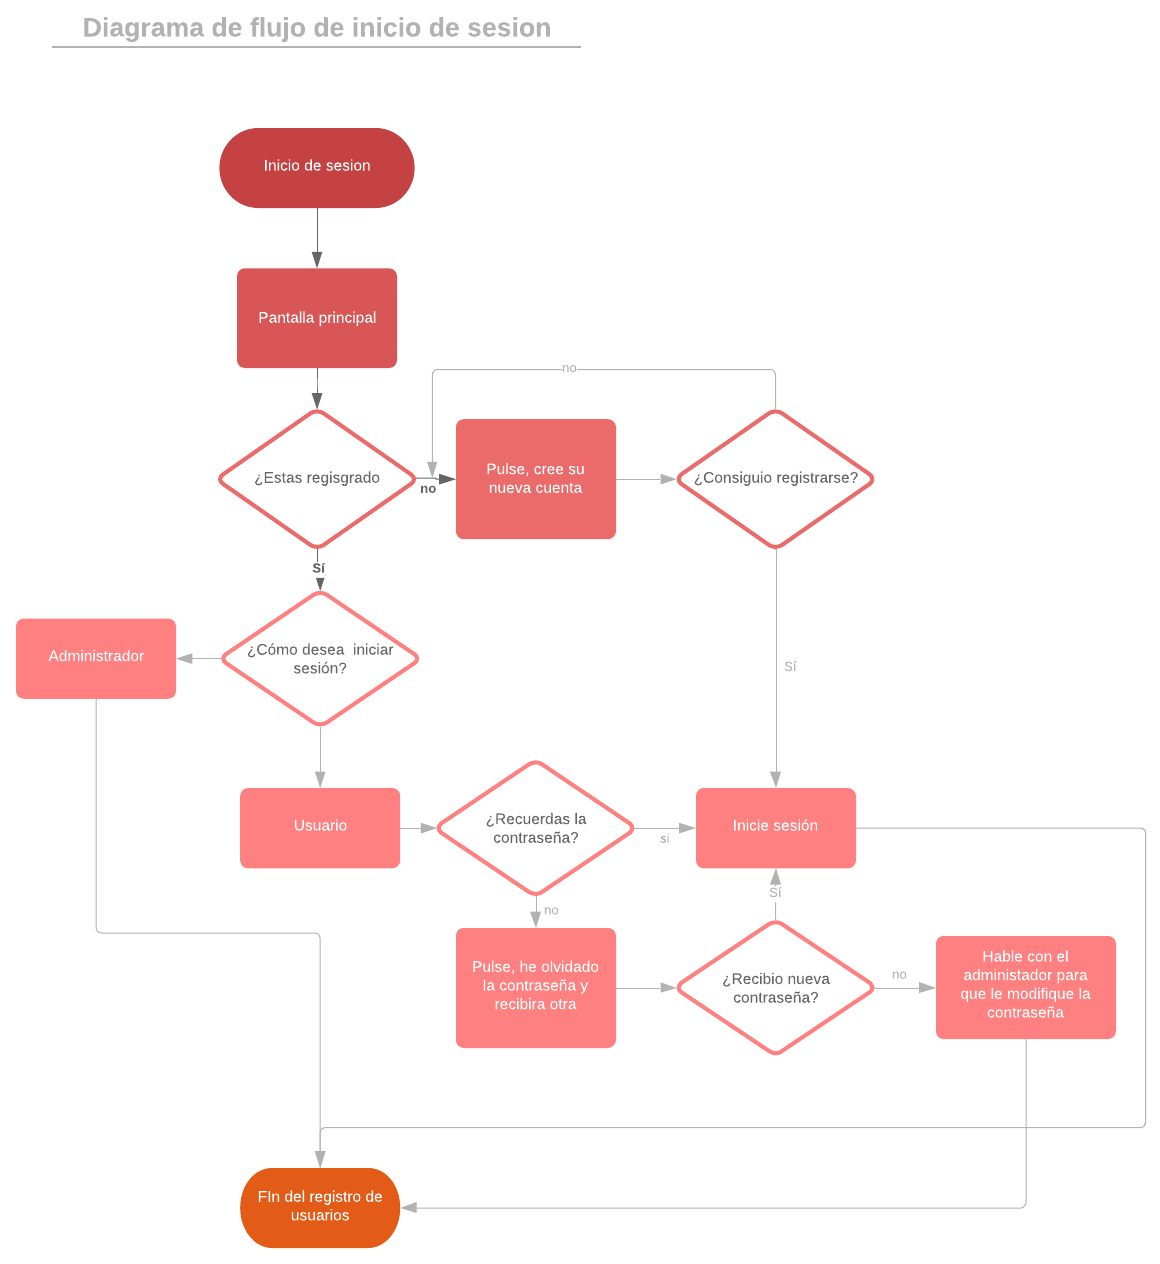
\includegraphics[width=0.60\textwidth]{diagramaFlujo}
    \caption{Diagrama de flujo de inicio de sesión}
    \label{fig:diagrama}
\end{figure}

En la siguiente imagen mostraremos el funcionamiento de la página una vez, hemos registrado sesión, dependiendo de si estamos en modo administrador o modo usuario \ref{fig:funcionamiento}.

\begin{figure}[H]
    \centering
    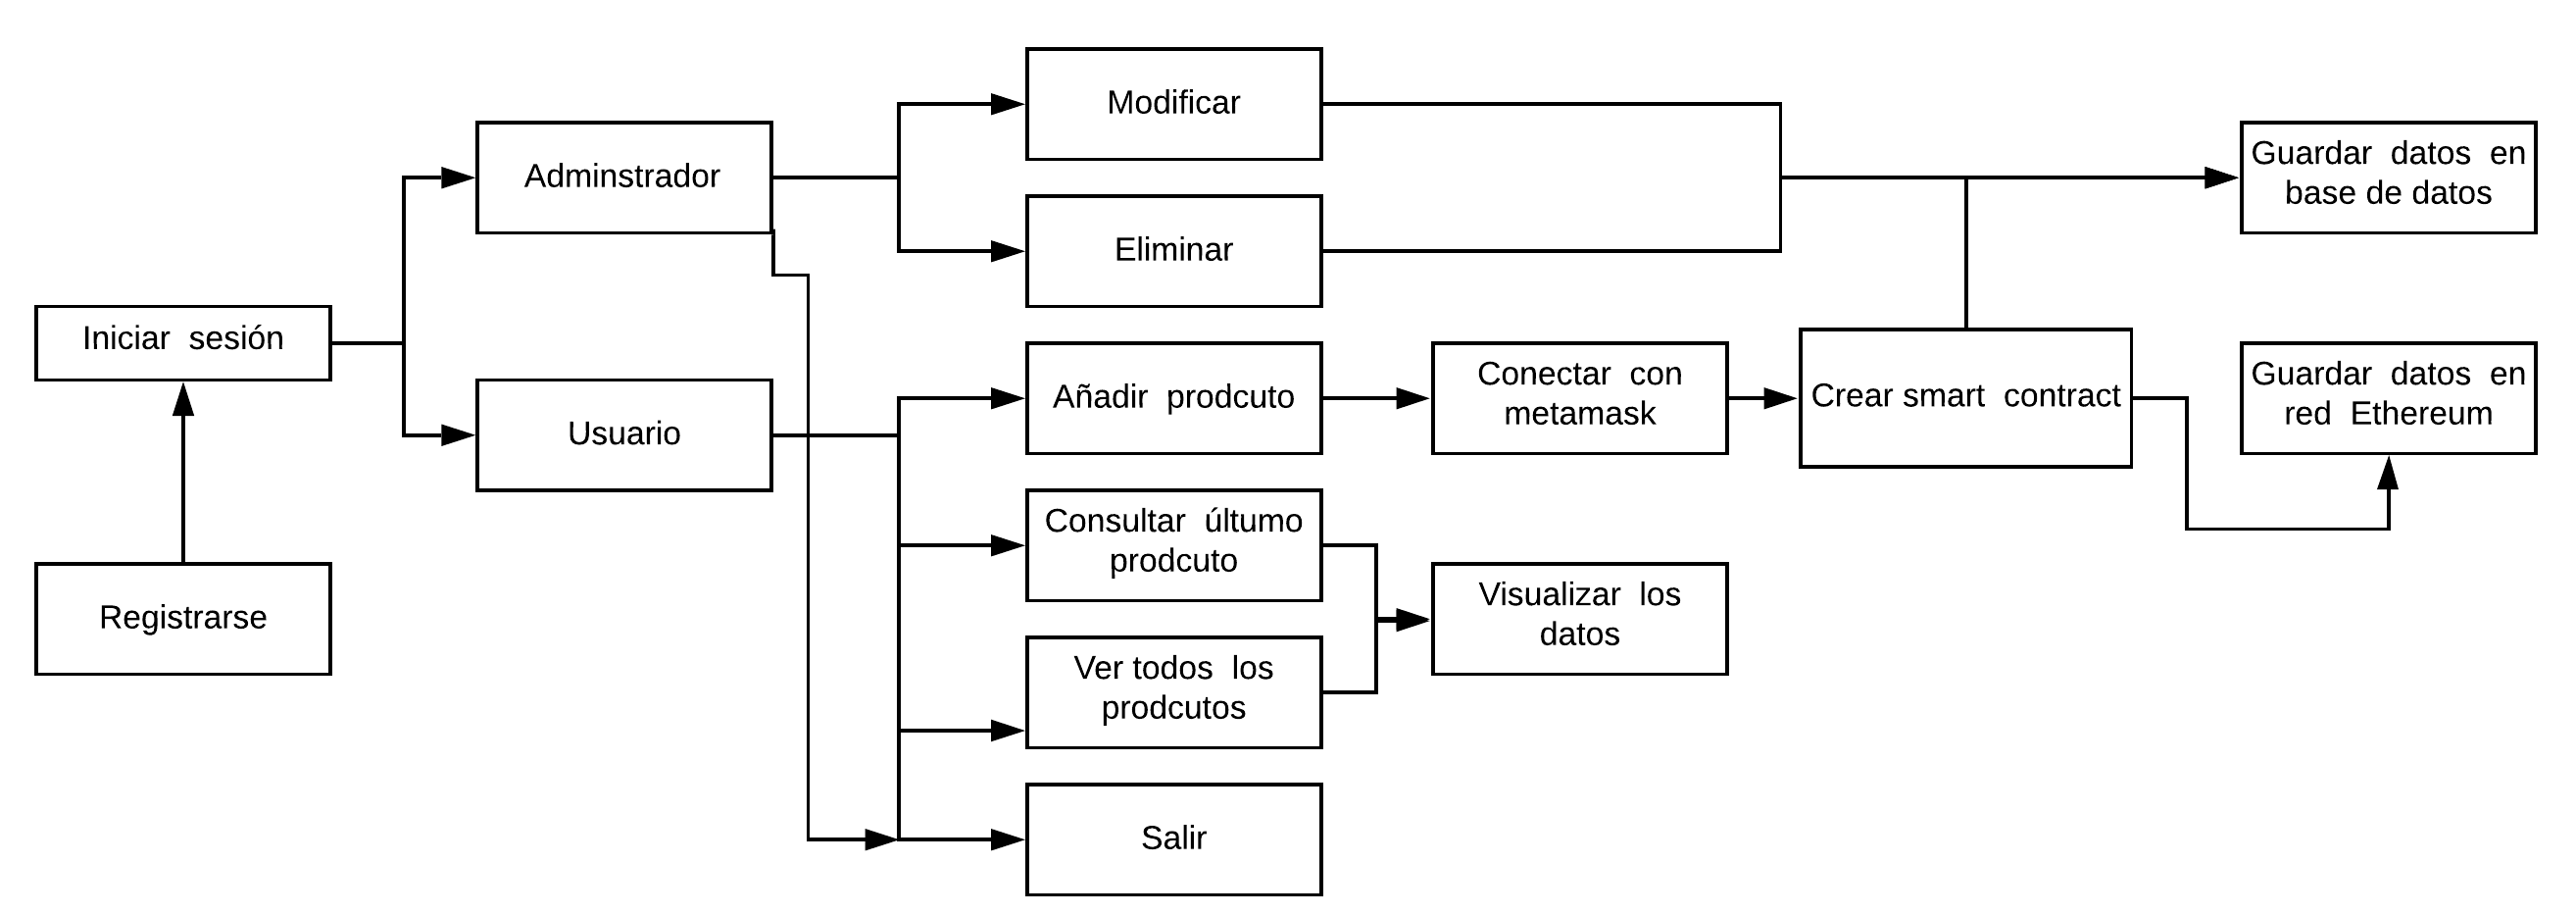
\includegraphics[width=1.00\textwidth]{funcionamientoPag}
    \caption{Tabla de productos}
    \label{fig:funcionamiento}
\end{figure}

A continuación, explicaremos las funciones que coinciden del usuario y del administrador:

\begin{enumerate}
	\item \textbf{Modificar}:
	\begin{itemize}
		\item \textit{Usuario}: podrá cambiar tanto el nombre y la contraseña de su propio usuario.
		\item \textit{Administrador}: tendrá acceso a cambiar el nombre y contraseña de todos los usuarios registrados en la base de datos, también podrá acceder a ver el id de los usuarios.
\end{itemize}			
\item \textbf{Eliminar}:
	\begin{itemize}
		\item \textit{Usuario}: dispondrá de una opción para eliminar su propia cuenta y todos los productos asociados a él.
		\item \textit{Administrador}: tendrá acceso a visualizar todos los usuarios registrados en la base de datos y podrá eliminar los que desee, esto también elimina todos los productos asociados previamente.
	\end{itemize}			
\item \textbf{Salir}:
	\begin{itemize}
		\item \textit{Usuario y administrador}: podremos salir una vez estemos registrado en la página web.
	\end{itemize}			
\end{enumerate}

\section{Diseño arquitectónico}

Para la creación de la interfaz de usuario, los requisitos que deseábamos cumplir eran facilidad y sencillez a la hora de usar la página web. La interfaz es clara y  limpia, con esto se consigue facilitar la interacción con el usuario. Esto se logra gracias a las páginas de estilo (css) y utilizando los \textit{bootstrap} que resulta en que la página quede con buen aspecto visual.
%\begin{figure}[H]
%	\begin{minipage}[b]{1.00\linewidth}
%		\centering
%		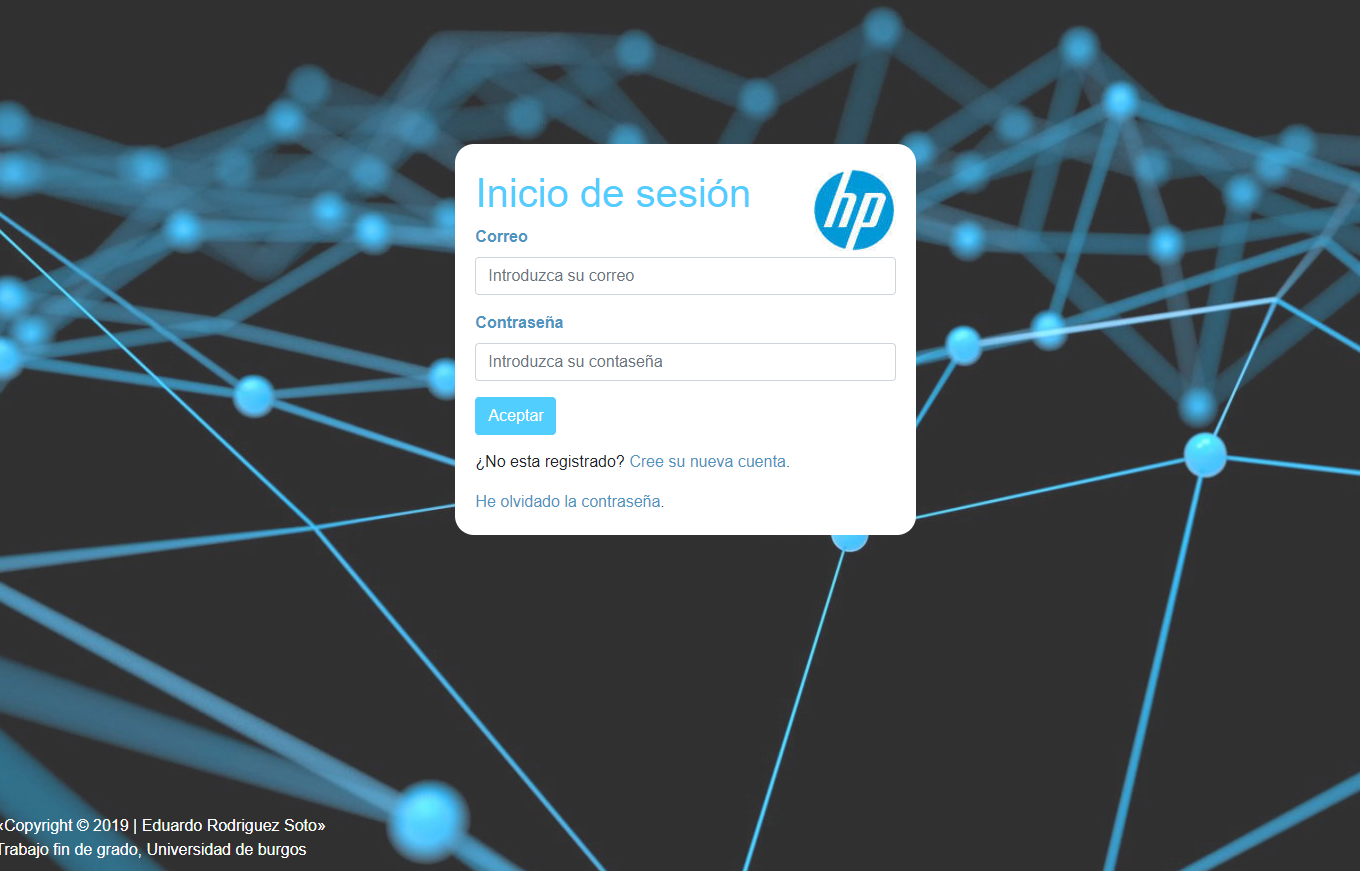
\includegraphics[width=1.00\textwidth]{incioPag}
%		\caption{Inicio de sesión}
%		\label{fig:inicio}
%	\end{minipage}
%	\hspace{0.3cm}
%	\begin{minipage}[b]{1.0\linewidth}
%		\centering
%		
\includegraphics[width=1.00\textwidth]{index}
%		\caption{Usuario registrado}
%		\label{fig:registrado}
%	\end{minipage}
%\end{figure}

En el apéndice \ref{ref:front} realizaremos la explicacion del \textit{front-end} de la aplicación final, para que el usuario pueda tener una guía explicativa. 

Con el objetivo de ayudar al usuario, hemos incorporado mensajes de aviso, tanto si son de error \ref{fig:error}, si son informativos \ref{fig:correcto} o son preguntas de confirmación \ref{fig:confirmar}.

\begin{figure}[H]
	\begin{minipage}[b]{0.5\linewidth}
		\centering
		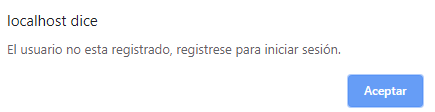
\includegraphics[width=1.00\textwidth]{error}
		\caption{Mensaje correo no registrado en la base de datos}
		\label{fig:error}
	\end{minipage}
	\hspace{0.3cm}
	\begin{minipage}[b]{0.5\linewidth}
		\centering
		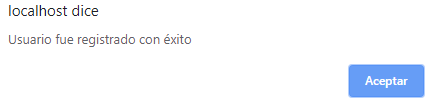
\includegraphics[width=1.00\textwidth]{correcto}
		\caption{Mensaje de usuario creado con éxito}
		\label{fig:correcto}
	\end{minipage}
	\\
	\begin{minipage}[b]{0.5\linewidth}
		\centering
		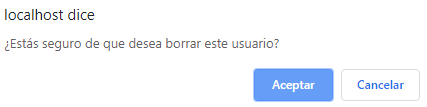
\includegraphics[width=1.00\textwidth]{confirmar}
		\caption{Mensaje de confirmar proceso}
		\label{fig:confirmar}
	\end{minipage}
\end{figure}





